\chapter{Základní problematika virtualizace síťových funkcí}

Tato kapitola se zabývá základní problematikou virtuálních síťových funkcí. Pro pochopení konceptu virtuálních síťových funkcí je nejprve nutvé vysvětlení několika základních pojmů a oblastí se kterou se souvisí. Proto jsou v této kapitole postupně popsány základní principy virtualizace, cloud computingu, softwarově definovaných sítí a následně již samotná oblast virtualizace síťových funkcí.


Co je to VNF a NFV. 


\section{Princip virtualizace}

Virtualizace je hlavní technologie, která umožnila vývoj nových řešení používaných v moderních datových centrech po celém světě. 
Základní pojmy. 

Virtualní stroj (VM)

Hypervizory

Host OS

Guest OS

Přestože cíl virtualizace je vždy stejný, tak existuje více přístupů, jak ho dosáhnout. V praxi se dnes používají tyto 2 hlavní metody virtualizace:

\begin{itemize}

\item Úplná virtualizace
\item Částečná virtualizace
\item Paravirtualizace

\end{itemize}

Typy hypervizorů:
\begin{itemize}
\item Typ 1 - nativní (Bare-metal)
\item Typ 2 - hostovaný
\end{itemize}


\begin{figure}[h]
\begin{centering}
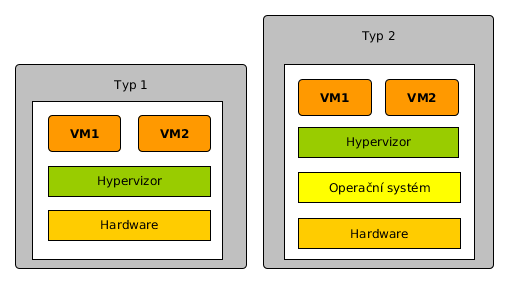
\includegraphics[scale=0.5]{images/virtualization}
\par\end{centering}
\caption{Základní znázornění virtualizace\label{fig:virtualization}}
\end{figure}


\section{Cloud computing}\label{sub:interaction}

Cloud Computing je hlavní oblast, která virtualizaci využívá. Z tohoto důvodu bude v této práci stručně vysvětlen. 

Obrázek cloudu.


\subsection{Model nasazení}

Existuje několik modelů, které určují, jak může být cloud nasazen. Tyto modely jsou vždy závislé na uživatelských požadavcích a potřebách. Uživatel za základě těchto parametrů může vybírat z těchto čtyř možných modelů pro nasazení cloudu.
\begin{itemize}
\item Privátní cloud
\item Veřejný cloud
\item Hybridní cloud
\item Komunitní cloud
\end{itemize}

Privátní cloud je cloudové prostředí vytvořené pro jednu organizaci. 

Veřejný cloud je cloudová infrastruktura, která je k dispozici k užívání veřejnosti. 

Hybridní cloud je 

Posledním modelem nasazení je komunitní cloud. V tomto modelu je 

\subsection{Distribuční model}

SaaS

PaaS

IaaS

NaaS

\subsection{Výhody}

\section{Softwarově definované sítě}\label{sub:interaction}

Architektura sítí - virtualizace síťové infrastruktury a návrh nových protokolů

\section{Virtualizované síťové funkce}\label{sub:interaction}

\begin{itemize}
\item Router
\item Firewall
\item IPS
\item IDS
\item Load-balancer
\item ...
\end{itemize}

\begin{figure}[h]
\begin{centering}
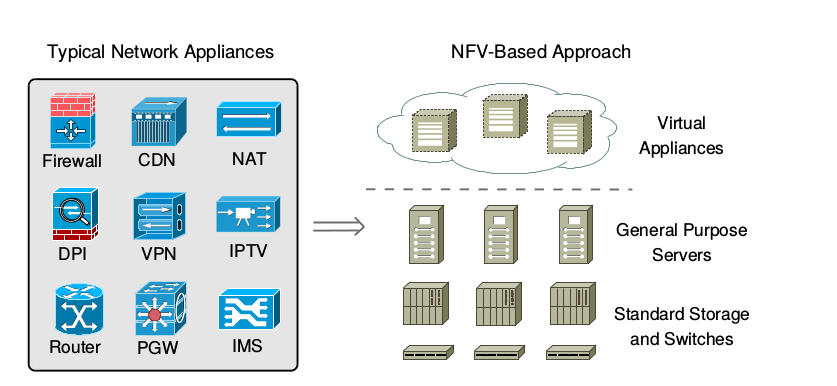
\includegraphics[scale=0.5]{images/vize_NFV}
\par\end{centering}
\caption{Vize Virtualizace síťových funkcí\label{fig:vize_NFV}}
\end{figure}

Tady bude napsaný rozdíl mezi tradičním HW přístupem a virtualizovaným přístupem

\subsection{Základní architektura}\label{sub:interaction}


\begin{figure}[h]
\begin{centering}
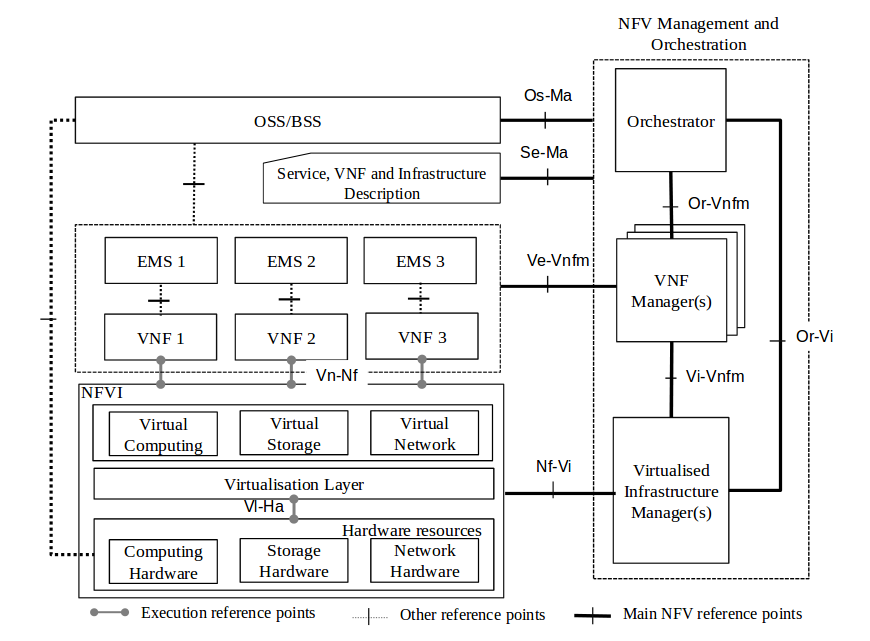
\includegraphics[scale=0.5]{images/NFV_architektura}
\par\end{centering}
\caption{NFV architektura\label{fig:NFV_architektura}}
\end{figure}

\subsection{Management a orchestrace}\label{sub:interaction}

Obrázek s popisem VNF frameworku

MANO
TOSCA a podobny hovna
